\documentclass[a4j,10.5pt,uplatex,twocolumn]{article}

\usepackage[dvipdfmx]{graphicx}
\usepackage[dvipdfmx]{color}
% \usepackage[top=30truemm,bottom=30truemm,left=25truemm,right=25truemm]{geometry}
\usepackage[top=30truemm]{geometry}

\title{Project Overview}
\author{Shoma Mori}
\date{\today}

\begin{document}

\maketitle

\section{Nodes}
There are two types of nodes in the system, namely, server and client.
Servers are basically validators, who verify transactions.
Clients are nodes who issue transactions.
Servers behave independently and so do clients, which means the system is asynchronous.

\section{Transactions}
The following is the flow that describes how a transaction from client $c_1$ to $c_2$ is approved by the system without a consensus.

\begin{enumerate}
    \item $c_1$ creates a transaction that indicates a payment from $c_1$ to $c_2$ using UTXO linked to $c_1$.
    \item $c_1$ sends the transaction to all servers.
    \item The servers verify the transaction by checking whether there are no conflicts with the history of transactions in their local storage.
    \item If not, the servers send $c_2$ the transaction with their own signatures which were generated from their private keys and add the transaction to the local storage.
    \item When $c_2$ receives the transaction, it verifies the signatures using the corresponding public keys.
    \item When $c_2$ receives valid signatures from more than two-thirds of all nodes, it regards the transaction to be approved.
    % \item The $c_1$ sends the transaction to $c_2$ with the signatures.
\end{enumerate}

\section{Double-spending}
Consider the situation that one client sends transactions that imply double-spending before none of them are not approved (Fig.~\ref{fig:double-spending-before}).
If a server receives more than one transaction of them, it can obviously detect double-spending.
If a server receives only one of them (meaning that the client tried so), the server may sign that transaction.
However, since the clients cannot send more than one transaction to 2/3 of all nodes without overlapping, more than one transaction cannot be approved.
In that case, only one of them would be approved in the best case, and no transactions are approved in the worst case.

\begin{figure}[tbp]
    \begin{center}
        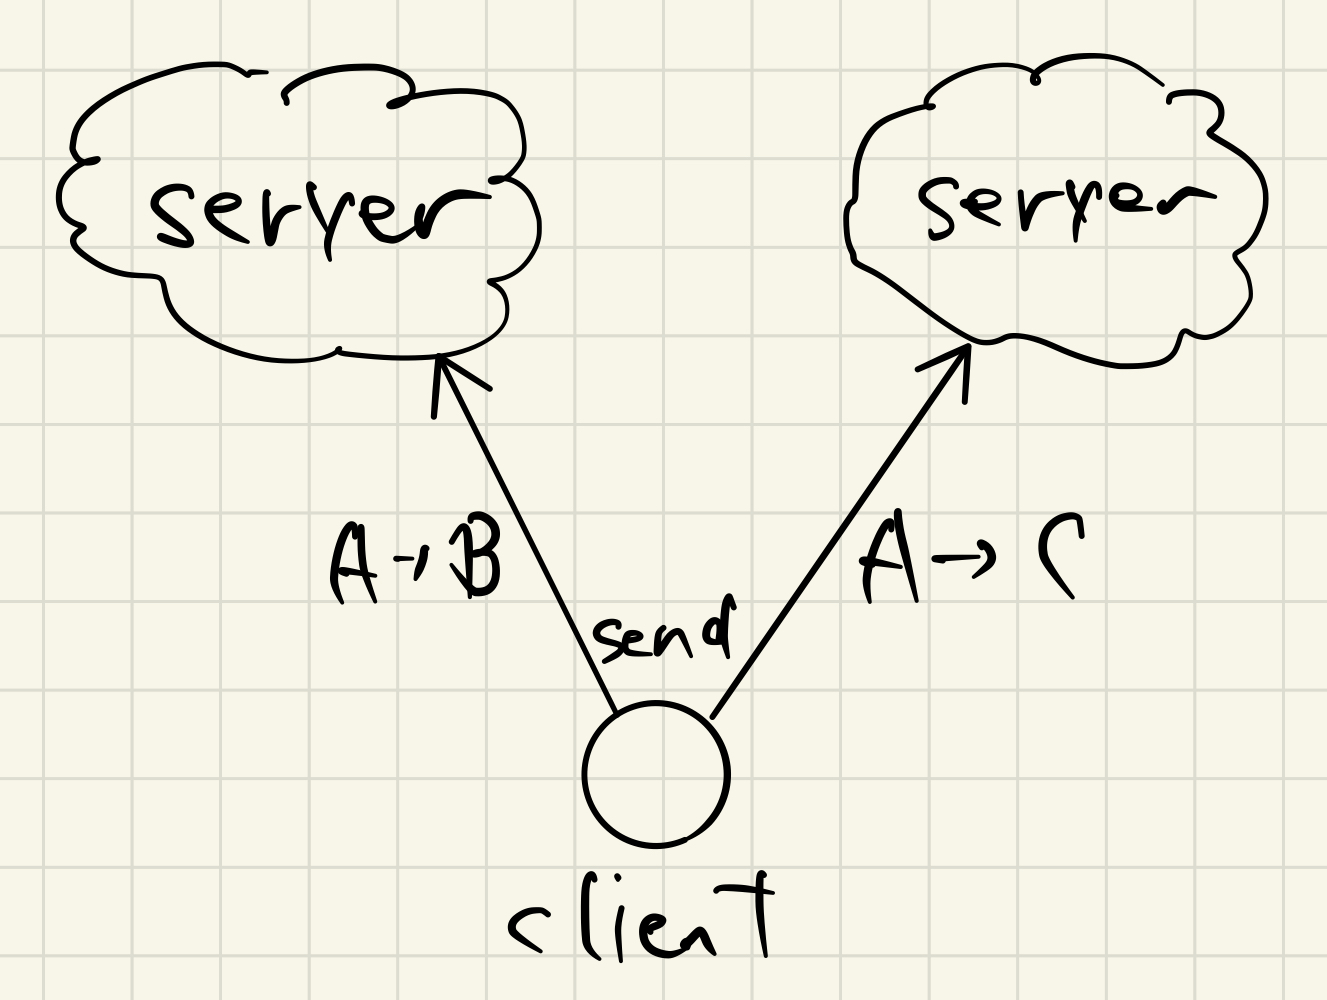
\includegraphics[width=5.0cm]{./fig/double-spending-before.jpeg}
        \caption{Double-spending}
        \label{fig:double-spending-before}
    \end{center}
\end{figure}

Next, consider that one client sends conflicting transactions after the conflicted transaction is approved (Fig.~\ref{fig:double-spending-after}).
In this case, servers can detect double-spending easily by checking their local storage and finding the conflicting transactions.

\begin{figure}[tbp]
    \begin{center}
        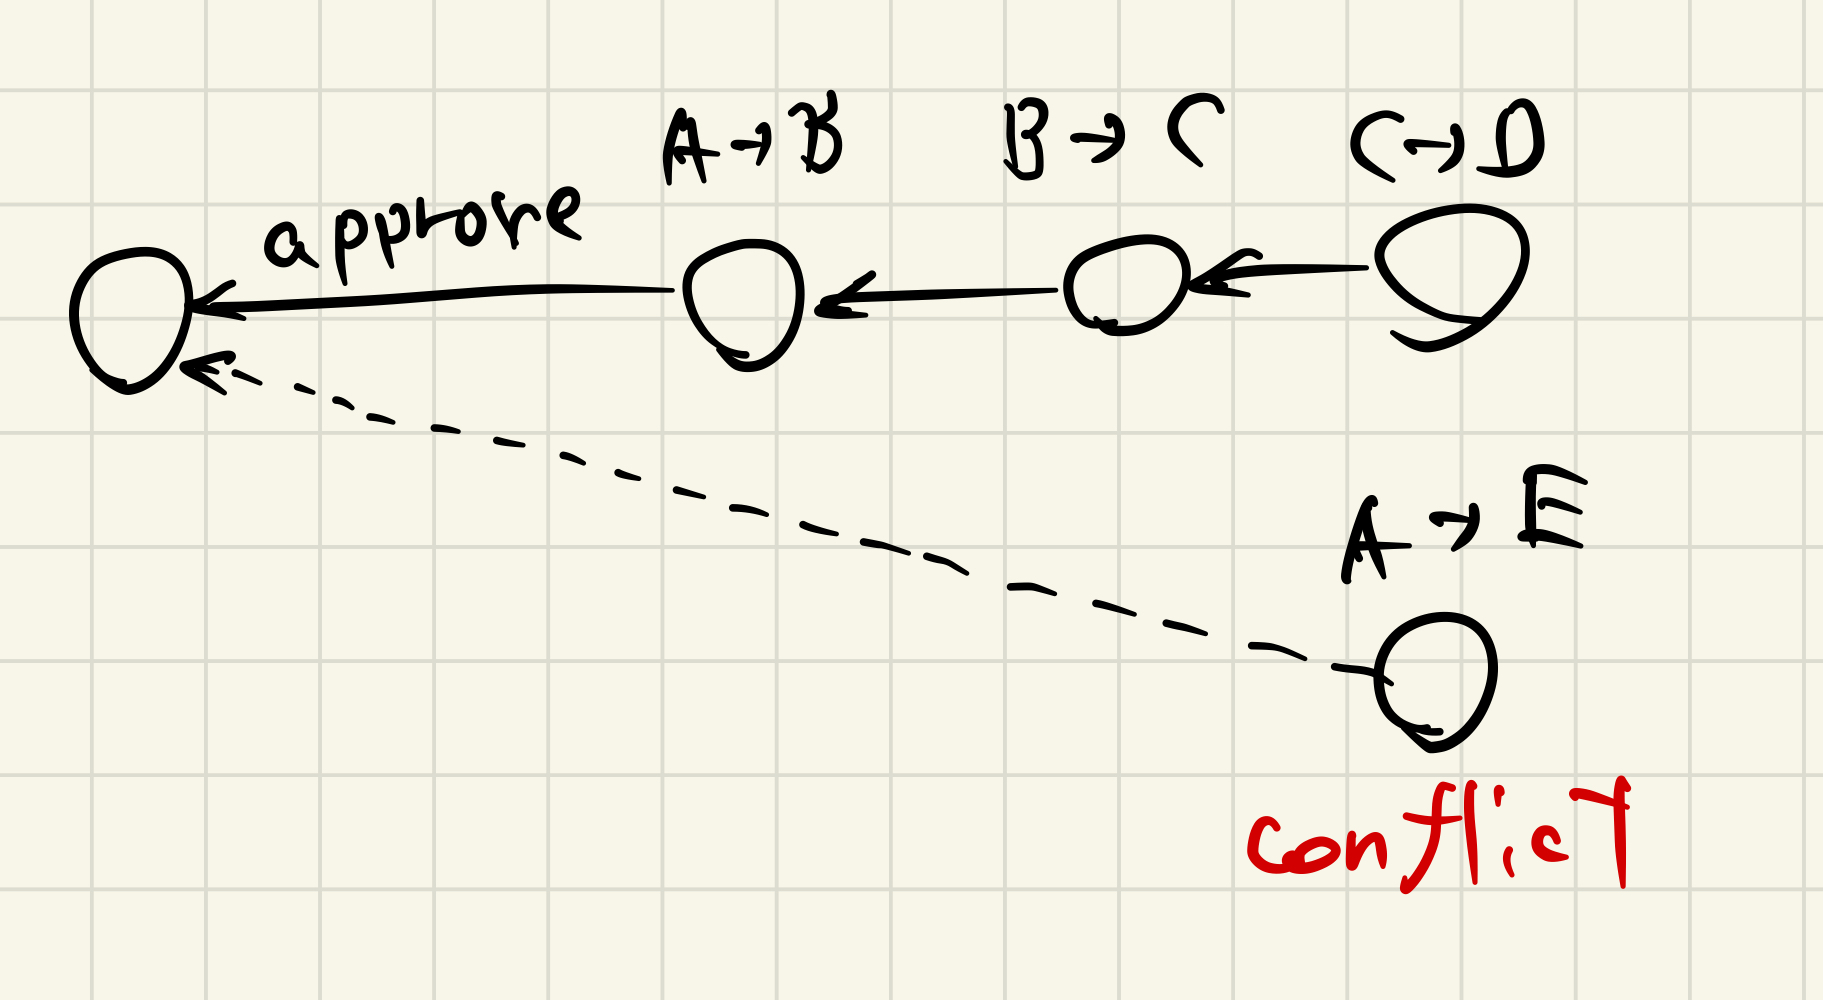
\includegraphics[width=5.0cm]{./fig/double-spending-after.jpeg}
        \caption{Double-spending}
        \label{fig:double-spending-after}
    \end{center}
\end{figure}



























\end{document}


